\begin{figure}[h]
		\begin{center}
			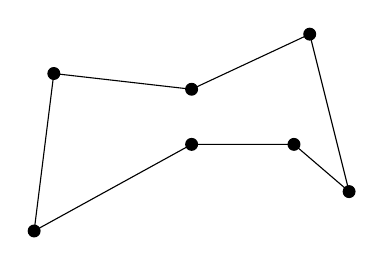
\begin{tikzpicture}
				\draw (0.0, 0.0) -- (0.25, 2.0) -- (2.0, 1.8) -- (3.5, 2.5) --
								  (4, 0.5) -- (3.3, 1.1) -- (2.0, 1.1) -- (0, 0);
			
				\draw[fill=black] (0, 0) circle (0.075);
				\draw[fill=black] (0.25, 2.0) circle (0.075);
				\draw[fill=black] (2.0, 1.8) circle (0.075);
				\draw[fill=black] (3.5, 2.5) circle (0.075);
				\draw[fill=black] (4, 0.5) circle (0.075);
				\draw[fill=black] (3.3, 1.1) circle (0.075);
				\draw[fill=black] (2.0, 1.1) circle (0.075);
			\end{tikzpicture}
		\end{center}
		\caption{Представление фигуры при помощи многоугольника}
	\end{figure}